At the date of writing, there are several implementations of encrypted databases.
Since the server is a part that cannot be fully trusted, most of the implementations are supposed to encrypt the data before it reaches the server. 
There are many levels of encryption, depending on how the data is encrypted and if it is all encrypted or only a part of it.
Another important aspect is how data is managed: in many cases data is only stored encrypted while all the process is done in cleartext, meanwhile some databases have implemented various algorithms for processing data in their encrypted form, so they don't have to manage cleartext.
According to these various methods we can divide them into 3 main categories:
\section{Data encryption at rest}
This type of encryption is also called TDE (Transparent Data Encryption) because is transparent to the user. 
The algorithm works by encrypting the database after the client ends the connection, and stores it to the disk ciphered, to prevent any malicious attacker from reading the database while it is not used. Of course, unless they recover the key. After that, it restores the database in plaintext only when the client needs to update it, so only in that moment the attacker can read it. A graphical representation of the algorithm is shown in figure 5. 
Encrypting data at rest has the advantage that one doesn't have to change the application level. In particular, all the applications that execute queries over the database remain the same. 
This means that all the data is in cleartext while the computation is done and, most important thing, while it is being sent through the network. This implies that any malicious eavesdropper can read any query or data retrieved and use it for his purposes.  
The first TDE implementation was done by Microsoft in SQL Server 2008 \cite{microsoft}.
Following Bill Gates's company, IBM \cite{ibm} and Oracle \cite{oracle} have implemented their own encrypted databases of this type. 
The company with headquarters in New York has implemented a software co-related with DB2, while Oracle has upgraded his own database.
Due to the passage of cleartext over the network this implementation is not related to our work, despite this type of database is widely used, since is the most transparent and quick encryption for a database. 
The interesting thing about this type of encryption is that can be integrated to record/column encryption, so it can add more security to the database (but increases the query time because of the double encryption). An implementation like the last one was done by Google\cite{google}.
Such algorithm can also be used for encrypting filesystems, like has done Windows with EFS\cite{efs}.\\
\begin{figure}[]
	\centering
	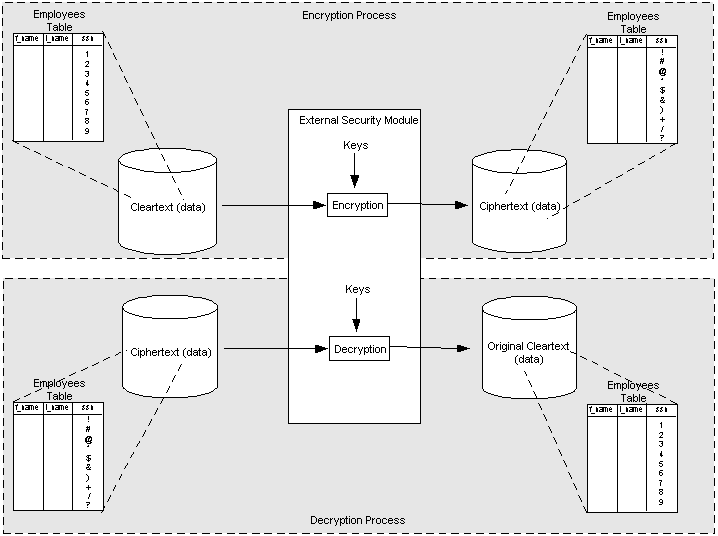
\includegraphics[scale=0.55]{transdata.png}
	\\Figure 1: A graphical representation Transparent Data Encryption (source www.oracle.com)
\end{figure}
\newpage


\section{Data encryption in transit}
The second method for encrypting data is to encrypt them "in transit", that means all the computation is done in plaintext. The advantage is that since the computation occurs client side, the data is encrypted before it is sent to the server, so all the packages that go through the network are ciphered, so if an eavesdropper recovers them, they cannot use them for malicious purposes.
This implementation relies on ciphering the single column of the database or, as it is in our case, single cells/records of it.
This method is widely used for filesystems, but today many companies are implementing it in their databases, since this ensure the client more security.
With data encryption in transit we have a reduction of the computation in the server.
The algorithm however must not be confused with public key cryptography, because with the last one the server has to decrypt the data. 
This method has been studied in the USA by \cite{cina}.


\section{Data encryption in use}
The last method relies on manage encrypted data, this means as soon as the data is inserted by the user it is encrypted in a particular manner. This allows the server to retrieve the data although it is encrypted. The implementation of this databases relies on homomorphic encryption, which is a type of encryption that allows manipulation over encrypted data\cite{homo1}\cite{homo2}. It has been studied in various articles, like \cite{tamper} and \cite{hard}.

\section{Our Approach}
Our approach is based on the data encryption in transit. In fact we encrypt all the packets before sending them to the server. The only information that the server have in plaintext are: the length of the data received and the initialization vector. Since this last is different for each encryption it must be added to the data. Other information that the server can retrieve are the level of the sector in the tree, but cannot reconstruct it. 